
\begin{figure}
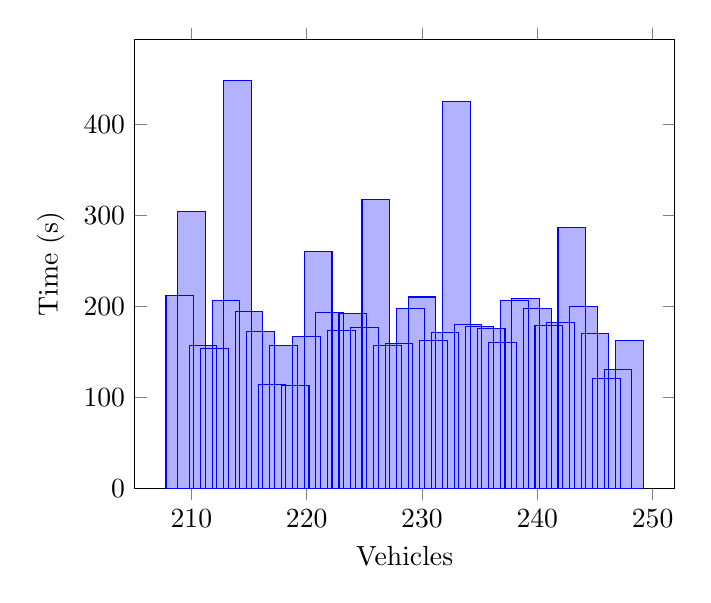
\begin{tikzpicture}
\begin{axis}[
legend style={anchor=west},
xlabel=Vehicles,
ylabel=Time (s),
ymin=0,
ybar,
]
\addplot coordinates {
(238, 206)
(239, 208)
(234, 180)
(235, 178)
(236, 175)
(237, 160)
(230, 210)
(232, 171)
(233, 425)
(245, 170)
(244, 200)
(247, 130)
(246, 120)
(241, 179)
(240, 197)
(242, 182)
(248, 162)
(209, 212)
(215, 194)
(222, 193)
(219, 113)
(214, 448)
(231, 162)
(216, 172)
(217, 114)
(212, 153)
(213, 206)
(210, 304)
(211, 157)
(218, 157)
(243, 286)
(229, 197)
(228, 159)
(227, 157)
(226, 317)
(225, 177)
(224, 192)
(223, 173)
(221, 260)
(220, 167)
};

\end{axis}
\end{tikzpicture}
\label{tik:time:100:98}
\caption{100 percent diving with GSC on route $98$}
\end{figure}
